\documentclass{article}
%\usepackage{amsmath}
%\usepackage{amssymb}
\usepackage{calc}
%\usepackage{caption}
\usepackage{color}
%\usepackage{commath}
%\usepackage{enumitem}
\usepackage{fancyhdr}
%\usepackage{float}
\usepackage{geometry}
\usepackage{graphicx}
\usepackage{hyperref}
\usepackage{lastpage}
%\usepackage{listings}
%\usepackage{mathtools}
\usepackage{pdfpages}
%\usepackage{siunitx}
%\usepackage{tikz}
\usepackage[disable]{todonotes}

\geometry{hmargin=2cm,vmargin=2cm}

\newcommand{\splitit}[2]{
    \noindent
    \begin{minipage}[t]{0.5\textwidth}
        #1
    \end{minipage}
    \begin{minipage}[t]{0.5\textwidth}
        #2
    \end{minipage}
}

\newcommand{\osscontrib}[3]{\item[#1] #2\hfill\\See #3.}


\begin{document}

\begin{center}
    {\Huge Taran Lynn}\\
    \vspace{0.25em}
    \hrule
    \vspace{0.25em}
    taranlynn0@gmail.com --- (707) 372-3259
\end{center}

\section*{Objective}

Seeking full time software engineering position specializing in low-level
systems, machine learning, and networking.

\section*{Education}

\begin{itemize}
    \item 2019 BS in Computer Science and Engineering from U.C. Davis
        (GPA 3.985).
\end{itemize}

\section*{Important Sites}

\begin{tabular}{ll}
    Personal & \url{http://lambda-11235.github.io/}\\
    GitHub & \url{https://github.com/lambda-11235/}\\
    LinkedIn & \url{https://www.linkedin.com/in/taran-lynn/}\\
\end{tabular}


\section*{Projects}

\begin{description}
    \item[Model Predictive Congestion Control]
        This is an ongoing research project to develop a new TCP congestion
        control algorithm that provides a smooth signal across dedicated WANs.
        To do this the algorithm employs concepts from model predictive control
        theory.
        The algorithm also allows users to dynamically set pacing rates on a per
        flow basis.
        Implementations have been developed for both the TCP congestion control
        and qDisc layers in the Linux kernel.
        Initial results have also been presented to ESnet members.
%I have been employed since the summer of 2018 (over a year) by U.C. Davis as a
%researcher.
%This research position involved working with Professors Dipak Ghosal and
%Nathan Hanford on a new model predictive congestion control algorithm for TCP.
%Two facets of this research involved implementing the algorithm in the Linux
%kernel and testing it over a 10 Gbps link to ES Net's test nodes.
%As part of this research I gave a talk to ES Net members at the Lawrence
%Berkley National Laboratory.

    \item[Randomizing Malloc for Security]
        This project aimed to disrupt certain classes of buffer overflow attacks
        that target malloc metadata.
        Such attacks require malloc to allocate memory chunks in a contiguous,
        predictable order.
        To counteract this we randomized the spacing between the chunks, which
        also had the effect of randomizing allocation order in some cases.
        We submitted a paper detailing the modification to the Hawaii
        International Conference on System Sciences (HICSS) in Spring of 2019.
        For reference the paper was entitled ``Randomizing Malloc: Stomp the
        Script Kiddies.''

    \item[Warcraft II Clone]
        This was a quarter long project for a software engineering class.
        It aimed to clone Warcraft II from abandon-ware.
        I worked in the multiplayer team.
        Our task was to implement the networking and game logic necessary to
        host online multiplayer matches.

    \item[Tesseract Training]
        This was a quarter long project for a machine learning class.
        Our team worked on training the Tesseract OCR engine to improve its
        accuracy when scanning a large set of wine catalog images provided by
        U.C.  Davis.
        The ultimate goal was to help them convert their catalogs to an online,
        searchable text.

    \item[IoT Sound Analysis]
        My team developed an IoT application on Texas Instrument's CC3200.
        This application used AWS Lambda to perform a Fast Fourior
        Transform on sampled audio data, which was then displayed as a
        heat plot on an OLED display on the CC3200.
\end{description}


\section*{Open Source Contributions}

\begin{description}
    \osscontrib{Idris}{I wrote documentation on the codata keyword.}{\url{https://github.com/idris-lang/Idris-dev/pull/3094/}}

    \osscontrib{NixOS}{I added a package for Red Eclipse to their
    repository.}{\url{https://github.com/NixOS/nixpkgs/pull/60952/}}
    \todo[inline]{Update when merged or new packages are submitted.}

    \osscontrib{The Secret Chronicles of Dr. M}{I helped port the game
    from SDL to SFML.}{\url{https://secretchronicles.org/en/}}

    \osscontrib{Red Eclipse}{I contributed custom content to their community
    repository.}{\url{https://www.redeclipse.net/}}
\end{description}

\subsubsection*{Personal Open Repos}

\begin{description}
    \item[TTyped] A dependently typed language directly based off of
        Coquand's Calculus of Constructions.

    \item[debtTools] A command line python program to help users track
        and calculate payments for compound interest debt.
        Also includes a paper that derives key formulas from first
        assumptions.

    \item[Markov's Password] A random password generator based off of
        the XKCD comic ``Password Strength''
        (\url{https://www.xkcd.com/936/}).
        It uses a variation of Markov chains to generate a sequence of
        random, made up, and pronounceable words.
        A version that uses a Hidden Markov Model is also being worked
        on.

    \item[FarRP] A library for functional reactive programming that
        leverages dependent types in the Idris.
        It is based on Neil Sculthorpe and Henrik Nilsson's paper "Safe
        Functional Reactive Programming through Dependent Types."
\end{description}


\section*{Notable Courses Taken}

\newcommand{\course}[2]{\fbox{#1 (#2)}}

\begin{minipage}{0.9\linewidth}
    \course{Algorithm Design}{ECS 122A/B}
    \course{Circuits I/II}{ENG 17/EEC 100}
    \course{Computer Architecture}{ECS 154A/B}
    \course{Embedded Systems}{EEC 172}
    \course{Machine Learning}{ECS 171}
    \course{Operating Systems}{ECS 150}
    \course{Parallel Architectures}{ECS 158}
\end{minipage}


\section*{Skills}

\begin{description}
    \item[Programming Languags (most to least experience)] \hfill\\
        \fbox{C}
        \fbox{C++}
        \fbox{Python}
        \fbox{Haskell}
        \fbox{Scala}
        \fbox{Java}
        \fbox{Lua}
        \fbox{Rust}
        \fbox{Coq}
        \fbox{Prolog}
        \fbox{Erlang}
        \fbox{Clojure}
        \fbox{Go}

    \item[Technologies Worked On] \hfill\\
        \fbox{Linux Kernel modules}
        \fbox{GNU C Library (glibc)}
        \fbox{Programming Language Interpreters}

    \item[Experience With] \hfill\\
        \begin{minipage}{0.9\linewidth}
            \fbox{Networking}
            \fbox{TCP Congestion Control}
            \fbox{Embedded Systems}
            \fbox{AWS (IoT \& Lambda)}
            \fbox{Control Systems}
            \fbox{Actor Model}
            \fbox{CSP Model}
            \fbox{Software Transaction Memory (STM)}
            \fbox{Functional Reactive Programming (FRP)}
        \end{minipage}
\end{description}


\section*{Awards}

\begin{itemize}
    \item Received 2019 UC David Computer Science Departmental Citation.
        \todo[inline]{Make clear what this is.}
\end{itemize}

\section*{References}

References can be provided upon request.

%\section*{Unofficial Transcript}
%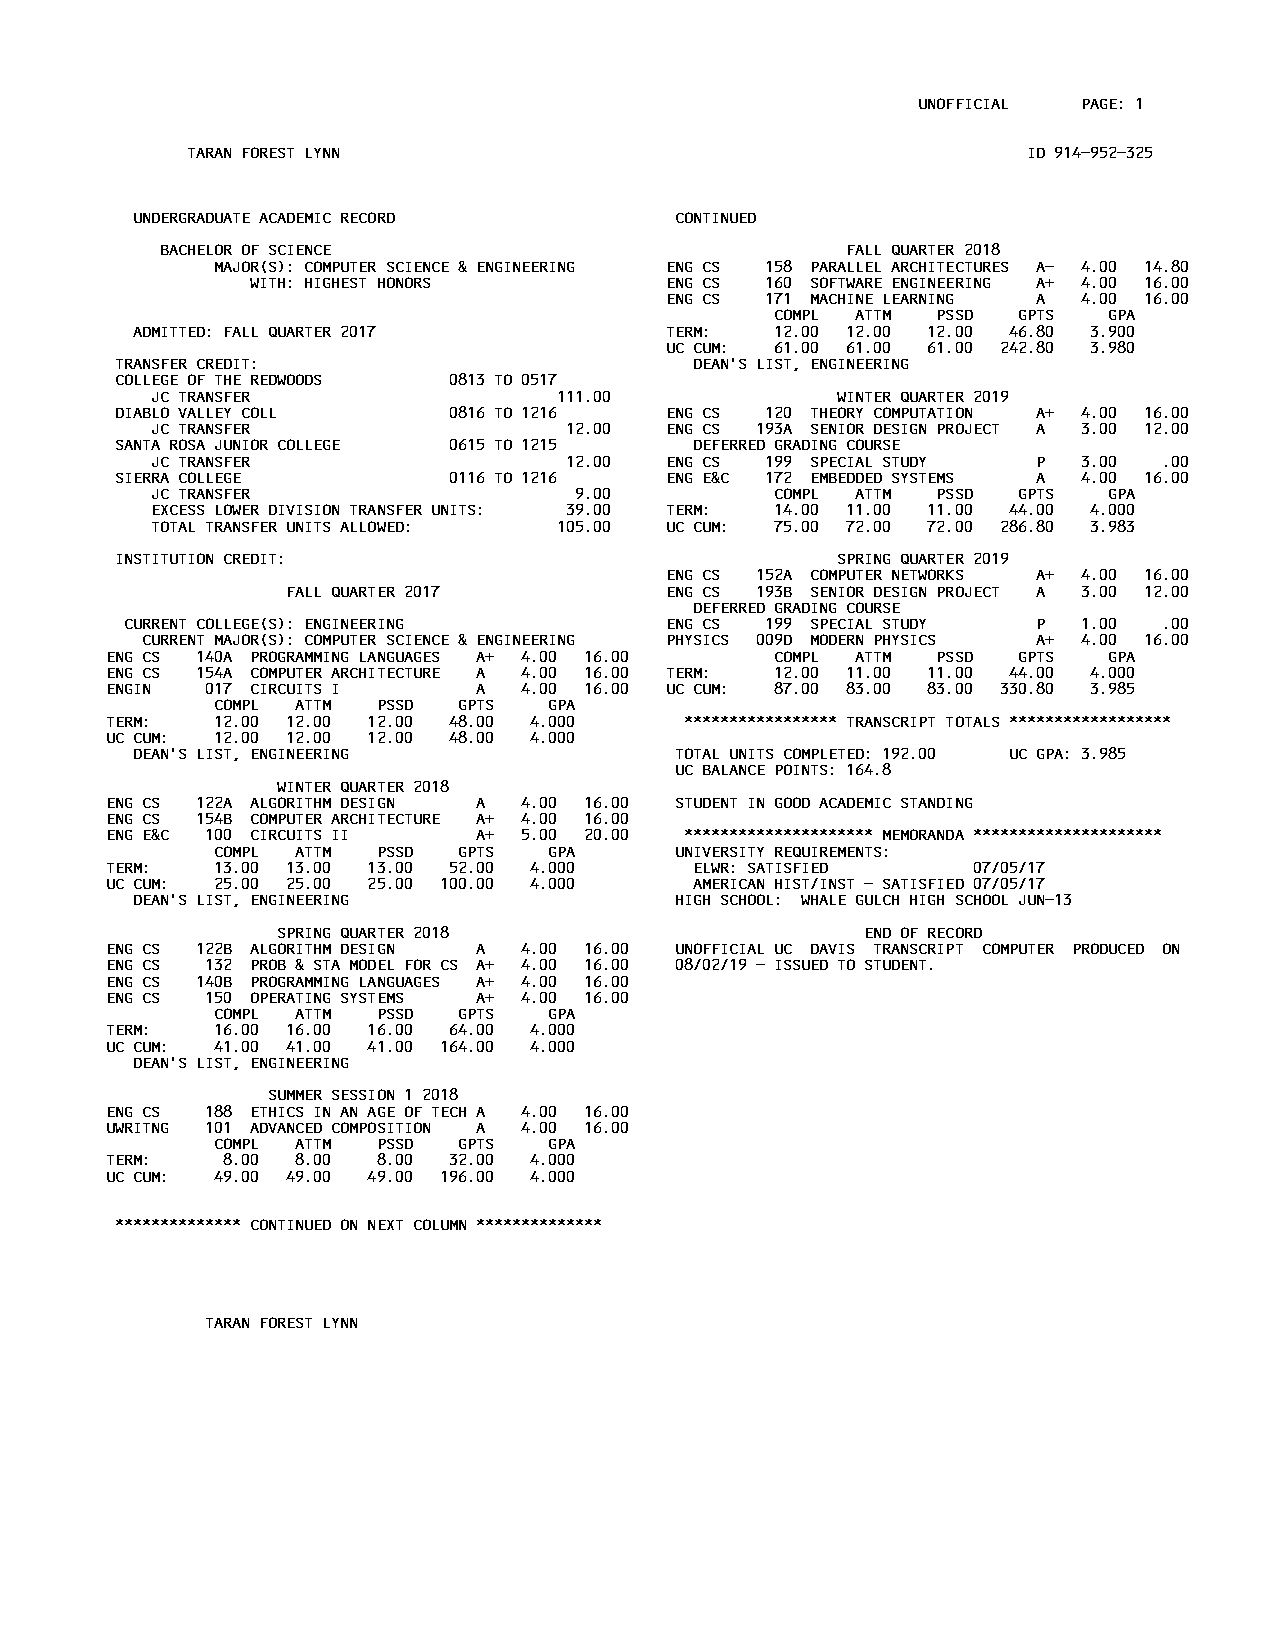
\includepdf{unofficial_trans.pdf}

\end{document}

